\vspace{-5pt}
\section{Preemption Point Placement Algorithm}\label{sec:implementation}

 Implementing a recursive algorithm directly from Equation~\ref{eqn:bbkwcet-cost} would lead to a computationally intractable implementation.  Instead, we now propose an \begin{math}O(N_i^{2})\end{math} dynamic programming algorithm for computing the optimal preemption points.  Our dynamic programming preemption point placement algorithm is summarized in Algorithm~\ref{alg:dynamic-optimal-ppp} shown below.  For each task $\tau_i$, we are given the following parameters: 1) the number of basic blocks $N_i$ , 2) the non-preemptive execution time of each basic block $b_i$, 3) the maximum allowable non-preemptive region $Q_i$, and 4) the preemption cost matrix $\xi_i$.  The preemption cost matrix $\xi_i$ is organized for each basic block \begin{math}\delta_{i}^{j}\end{math} and contains the preemption cost for all successor basic blocks of the task's control flow graph.  The minimum preemption cost up to all basic blocks is computed and stored in a matrix denoted $B_{i}$.  The $B_{i}$ matrix is initially seeded with the corresponding $q_i$ preemptive cost for basic block pairs that satisfy the constraint $q_{i}(\delta_{i}^{j},\delta_{i}^{k}) \leq Q_{i}$. All other entries are set to infinity.  As we consider whether each basic block $\delta_{i}^{k}$ is in the set of optimal preemption points, the location of the previous basic block $\delta_{i}^{j}$ with minimal preemption cost is stored in an array denoted $\rho_{prev}$.  The algorithm examines each basic block from \begin{math}\delta_{i}^{1}\end{math} to \begin{math}\delta_{i}^{N_i}\end{math} to minimize the preemption cost by traversing backwards from the current basic block $\delta_{i}^{k}$ under consideration in order to find the basic block $\delta_{i}^{j}$ with minimal preemption cost subject to the constraint $q_{i}(\delta_{i}^{j},\delta_{i}^{k}) \leq Q_{i}$.  While each basic block will have a predecessor with minimum preemption cost, the list of selected preemption points is obtained by starting with basic block $\delta_{i}^{N_i}$ and hopping to the predecessor basic block stored at $\rho_{prev}(\delta_{i}^{N_i})$, denoted $\delta_{i}^{m}$.  Basic blocks $\delta_{i}^{N_i}$ and $\delta_{i}^{m}$ are added to the optimal preemption point set $\rho_{i}$.  This basic block hopping process continues until basic block $\delta_{i}^{0}$ is reached.  The set $\rho_{i}$ contains the complete list of selected optimal preemption points.
{\fontsize{10}{10}\selectfont
\begin{algorithm}
\caption{D.P. Optimal Preemption Point Placement}
\label{alg:dynamic-optimal-ppp}
\begin{algorithmic}[1]
\small
\Function{$Select\_Optimal\_PPP$}{$N_{i}$,$b_{i}$,$Q_{i}$,$\xi_i$}
%\State {$C_{i}^{NP}\ \gets\ \infty\ q_{i}\ \gets\ \infty\ B_{i}\ \gets\ \infty\ \rho_{prev}\ \gets\ \{\delta_{i}^{0}\}$};
\State {$ B_{i}\ \gets\ \infty\ \rho_{prev}\ \gets\ \{\delta_{i}^{0}\}$};
\If {$b_{i}^{k} > Q_{i}\ for\ some\ k\ \in\ \{1,\ldots, N_{i}\}$}
\State\Return{INFEASIBLE;}
\EndIf
\State{$B_i(\delta_i^0)\ \gets\ 0$};
%\State{$C_{i}^{NP}(\delta_{i}^{0}$,$\delta_{i}^{0}) \gets\ 0$};
%\State{$q_i(\delta_{i}^{0}$,$\delta_{i}^{0}) \gets\ 0$};
\For{$k: 0\leq k\leq N_{i}$}
\State{$C_{i}^{NP}(\delta_{i}^{k}$,$\delta_{i}^{k}) \gets\ 0$};
\State{$q_{i}(\delta_{i}^{k},\delta_{i}^{k}) \gets\ 0$};
%\State\Call{$Compute\_PPCost$}{$\delta_{i}^{k-1}$,$\delta_{i}^{k}$};
\For{$j: k-1\geq j\geq 0$}
%\Comment{$Check\ preemption\ cost\ at\ BB\ \delta_{i}^{j}\ with\ preemption$}
%\Comment{$at\ BB\ \delta_{i}^{0}\ and\ BB\ \delta_{i}^{k}$}
%\State\Call{$Compute\_PPCost$}{$\delta_{i}^{0}$,$\delta_{i}^{j}$};
%\State\Call{$Compute\_PPCost$}{$\delta_{i}^{j}$,$\delta_{i}^{k}$};
\State{$C_{i}^{NP}(\delta_{i}^{j},\delta_{i}^{k}) \gets b_i^{j+1} + C_{i}^{NP}(\delta_{i}^{j+1},\delta_{i}^{k})$};
\State{$q_{i}(\delta_{i}^{j},\delta_{i}^{k}) \gets\ \xi_i(\delta_{i}^{j},\delta_{i}^{k}) + C_{i}^{NP}(\delta_{i}^{j},\delta_{i}^{k})$};
\If {$q_{i}(\delta_{i}^{j},\delta_{i}^{k}) \leq Q_{i}$}
\State{$P_{cost}\ \gets\ B_{i}(\delta_{i}^{j})\ +\ q_{i}(\delta_{i}^{j},\delta_{i}^{k})$};
\If {$P_{cost} < B_{i}(\delta_{i}^{k})$}
\State{$B_{i}(\delta_{i}^{k}) \gets P_{cost}$};
\State{$\rho_{prev}(\delta_{i}^{k}) \gets \delta_{i}^{j}$};
\EndIf
\EndIf
\EndFor
\EndFor
\State{$\rho_{i}\ \gets\ $\Call{$Compute\_PPSet$}{$N_{i},\rho_{prev}$}};
\State\Return{FEASIBLE;}
\EndFunction
\\
%\Function{$Compute\_PPCost$}{$\delta_{i}^{j}$,$\delta_{i}^{k}$}
%\If {$q_{i}(\delta_{i}^{j},\delta_{i}^{k})$ = $\infty$}
%\State{$Compute\ \xi_{i}(\delta_{i}^{j}$,$\delta_{i}^{k})\ using\ Equation\ (\ref{eqn:prempt-cost})$};
%\State{$Compute\ C_{i}^{NP}(\delta_{i}^{j}$,$\delta_{i}^{k})\ using\ Equation\ (\ref{eqn:c-np2})$};
%%\State{$Compute\ q_{i}(\delta_{i}^{j}$,$\delta_{i}^{k})\ using\ Equation\ (\ref{eqn:mthnpr-time})$};
%\State{$q_{i}(\delta_{i}^{j},\delta_{i}^{k}) \gets C_i^{NP}(\delta_{i}^{j},\delta_{i}^{k}) + \xi_i(\delta_{i}^{j},\delta_{i}^{k})$};
%%\If {$q_{i}(\delta_{i}^{j}$,$\delta_{i}^{k})\ \leq\ Q_{i}\ and\ \delta_{i}^{j}\ =\ \delta_{i}^{0}$}
%%\State{$B_{i}(\delta_{i}^{k}) \gets q_{i}(\delta_{i}^{j}$,$\delta_{i}^{k})$};
%%\State{$\rho_{prev}(\delta_{i}^{k}) \gets \delta_{i}^{j}$};
%%\Else
%%\If {$j-k\ =\ 1$}
%%\State\Return{INFEASIBLE;}
%%\EndIf
%%\EndIf
%\EndIf
%\EndFunction
\\
\Function{$Compute\_PPSet$}{$N_{i}$,$\rho_{prev}$}
\State {Computes $\rho_{i}$ from $\rho_{prev}$ (Details omitted)}
%\State {$\rho_{i}\ \gets\ \{\}$};
%\State {$\rho_{index}\ \gets\ \{\delta_{i}^{N_{i}}\}$};
%\While {$\rho_{index}\ \neq\ \delta_{i}^{0}$}
%\State {$\rho_{i}\ \gets\ \rho\ \cup \rho_{index}$};
%\State {$\rho_{index}\ \gets\ \rho_{prev}(\rho_{index})$};
%\EndWhile
%\State {$\rho_{i}\ \gets\ \rho_{i}\ \cup \rho_{index}$};
%\State\Return{$\rho_{i}$;}
\EndFunction
\normalsize
\end{algorithmic}
\end{algorithm}
}
%\showthe\floatsep 12pt
%\showthe\textfloatsep 20pt
%\showthe\intextsep 12pt

To exemplify how our algorithm works, consider the following example.
\begin{figure}[h!]
\vspace{-5pt}
\begin{center}
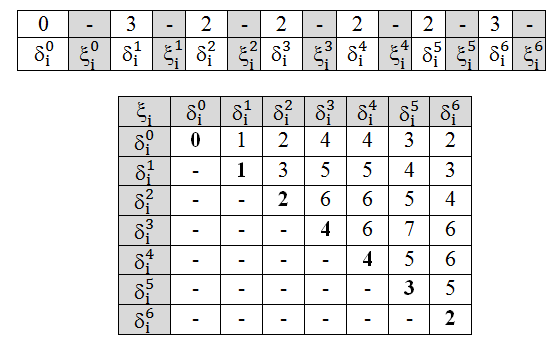
\includegraphics[width=0.45\textwidth]{algo_example.png}
\caption{Algorithm Example.}
\label{fig:algo_example}
\end{center}
\vspace{-10pt}
\end{figure}
Let $N_i=6$ and $Q_i=12$ for the following basic block structure with WCET and preemption costs shown in Figure~\ref{fig:algo_example}.  The algorithm computes and stores the cumulative non-preemptive execution costs for starting and ending basic block pairs in a matrix denoted $C_{i}^{NP}(\delta_{i}^{j}$,$\delta_{i}^{k})$. For example, $C_{i}^{NP}(\delta_{i}^{1}$,$\delta_{i}^{3})\ =\ b_{i}^{2}\ +\ b_{i}^{3}\ =\ 2\ +\ 2\ =\ 4$.  We don't include $b_{i}^{1}$ since the preemption occurs after execution of basic block $\delta_{i}^{1}$.  Using this information, the combined WCET and CRPD costs for each basic block pair is computed and stored in a matrix denoted $q_{i}$. For example, $q_{i}(\delta_{i}^{1}$,$\delta_{i}^{3})\ =\ C_{i}^{NP}(\delta_{i}^{1}$,$\delta_{i}^{3})\ +\ \xi_{i}(\delta_{i}^{1}$,$\delta_{i}^{3})\ =\ 4\ +\ 5\ =\ 9$.  The remaining $q_{i}$ matrix entries are computed in a similar fashion.  These matrices are shown in Figure~\ref{fig:algo_example_2}.  The shaded cells in the $q_{i}$ matrix represent cases where the combined WCET and CRPD costs for these basic block pairs exceed the maximum allowable non-preemptive region parameter $Q_i$.  During execution of the algorithm, the minimum combined WCET + CRPD costs are computed for each basic block and stored in an array denoted $B_{i}$.  Basic block pairs with preemptive costs that are less than or equal to $Q_i$ are candidates for selection.  When a lower cost is determined for a given basic block, the predecessor preemption point is updated in the $\rho_{prev}$ array which keeps track of the selected predecessor preemption points thereby forming a daisy chain containing the entire set of selected preemption points.  The final results are illustrated in Figures~\ref{fig:algo_example_2} and~\ref{fig:algo_example_3} below.
\begin{figure}[h!]
\vspace{-5pt}
\begin{center}
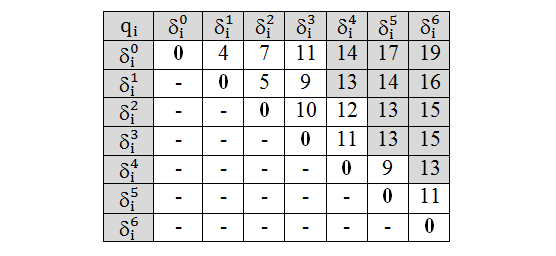
\includegraphics[width=0.45\textwidth]{algo_example_2.png}
\caption{Combined WCET and CPRD Costs.}
\label{fig:algo_example_2}
\end{center}
\vspace{-5pt}
\end{figure}
\begin{figure}[h!]
\vspace{-5pt}
\begin{center}
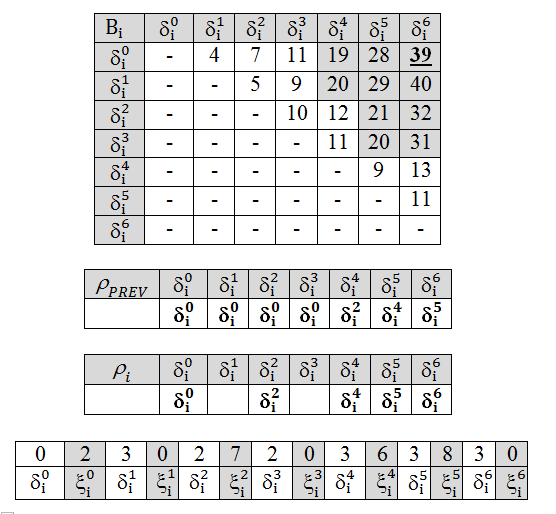
\includegraphics[width=0.45\textwidth]{algo_example_3.png}
\caption{Algorithm Results.}
\label{fig:algo_example_3}
\end{center}
\vspace{-10pt}
\end{figure}

The maximum blocking time \begin{math}Q_{i}\end{math} that each task may tolerate utilizes the computed task WCET parameter \begin{math}C_{i}\end{math}.  The method for obtaining the maximum blocking time is eloquently summarized for the Earliest Deadline First (EDF) and Fixed Priority (FP) scheduling by Bertogna et. al. algorithms~\cite{bertogna:11}~\cite{bertogna:10}.  The circular dependency between the maximum blocking time \begin{math}Q_{i}\end{math} and task WCET \begin{math}C_{i}\end{math} parameters suggests an iterative approach to allow the two parameters to convergence to a steady state.  One such iterative approach contains the following steps as given in Algorithm~\ref{alg:iterative-schedulability-optimal-ppp}.
%
%\begin{spacing}{2.0}
{\fontsize{10}{10}\selectfont
\begin{algorithm}
\caption{Iterative Schedulability and Preemption Point Placement Algorithm}
\label{alg:iterative-schedulability-optimal-ppp}
\begin{algorithmic}[1]
\small
\State{Start with a task system that may or may not be feasible.}
\State{Assume the CRPD of the task system is initially zero.}
%\Repeat
    \Repeat
        \State\begin{varwidth}[t]{\linewidth}
        Run the Baruah algorithm to obtain the maximum \par
        \hskip\algorithmicindent non-preemptive region $Q_i$ for each task.
        \end{varwidth}
        \State\begin{varwidth}[t]{\linewidth}
        Select optimal preemption points using our \par
        \hskip\algorithmicindent dynamic programming algorithm.
        \end{varwidth}
        \State\begin{varwidth}[t]{\linewidth}
        Compute the CRPD and the preemptive WCET \par
        \hskip\algorithmicindent $C_i$ from the selected preemption points.
        \end{varwidth}
    \Until{the selected preemption points do not change.}
%    \If{the task system is feasible/schedulable}
%        \State\begin{varwidth}[t]{\linewidth}
%        Increase the system utilization by decreasing the \par
%        \hskip\algorithmicindent periods via a binary search.
%        \end{varwidth}
%    \Else
%        \State\begin{varwidth}[t]{\linewidth}
%        Decrease the system utilization by increasing the \par
%        \hskip\algorithmicindent periods via a binary search.
%        \end{varwidth}
%    \EndIf
%\Until\begin{varwidth}[t]{\linewidth}
%the system utilization change is less than some \par
%\hskip\algorithmicindent tolerance.
%\end{varwidth}
%\State{The breakdown utilization is given by U.}
\normalsize
\end{algorithmic}
\end{algorithm}
}
%\end{spacing}
%\vspace{-10pt} 